
\subsection{Investigating Latent Representations in VCCA-private\texorpdfstring{$_{x i}$}{TEXT}}
\label{paperB:app:investigating_latent_representations_in_vcca_private_xi}

Figure \ref{paperB:fig:2d_visualizations_pca_vcca_private_xi} shows the shared and private latent spaces of VCCA-private$_{x i}$, as well as the latent space of the standard VCCA$_{x i}$ for comparison. Note that the shared latent spaces in Figure \ref{paperB:fig:2d_visualizations_pca_vcca_private_xi}(a) and \ref{paperB:fig:2d_visualizations_pca_vcca_private_xi}(b) have different structures mainly due to the different settings of their likelihood weight $\lambda_{i}$, which is $\lambda_{i} = 1000$ for VCCA$_{x i}$ and $\lambda_{i} = 10$ for VCCA-private$_{x i}$. We observe in Figure \ref{paperB:fig:2d_visualizations_pca_vcca_private_xi}(c) that the natural images are structured based on their similarities in background and camera setup. Across the upper right and the lower left parts of the cluster, we find images of grocery items closely packed together in bins. The middle and upper left part includes images with the hand of the photographer and grey backgrounds, e.g., the floor and shelves in the grocery store. Note that this private latent space is rather densely packed mainly because the KL divergence $\KL(q_{\phi_{x}}(u_{x} |x)\,||\,p(u_{x}))$ is steadily decreasing towards zero (see Figure \ref{paperB:fig:kl_divergence_vcca_private_with_iconic_image}(a)). This means that the approximate posterior $q_{\phi_{x}}(u_{x} |x)$ is collapsing to its prior distribution, which is why the mean values $\mu_{u_{x}}$ are close to the origin of the space. The mean values $\mu_{u_{i}}$ for the private latent variable $u_{i}$ are shown in Figure \ref{paperB:fig:2d_visualizations_pca_vcca_private_xi}(d) using the iconic image. Note that every iconic image $i$ is projected at the same location in the latent space. We observe that similar iconic images are projected close to each other. For instance, an orange, grapefruit and yellow bell pepper have been projected in the upper part, packaged items are in the center parts and the left region we find round objects with a dark red color. To the far right, we see a green and a red apple that has been pushed far away from the similar iconic images on the left. If we look closer into these iconic images, we observe that the apples on the right have a higher stalk on top of the apple than the apples on the left side has, which could be the reason why the model has separated them in the latent space. Another interesting observation is that iconic images with multiple items, e.g., tomatoes, kiwis and satsumas, have been projected into the lower region of the space. We conclude that similar iconic images, based on color and their appearance in the image, are grouped closely in the private latent space.  


\begin{figure}[th!]
	\centering
	\begin{minipage}{\textwidth}
		\centering
		\begin{subfigure}[t]{0.48\textwidth}
			\centering
			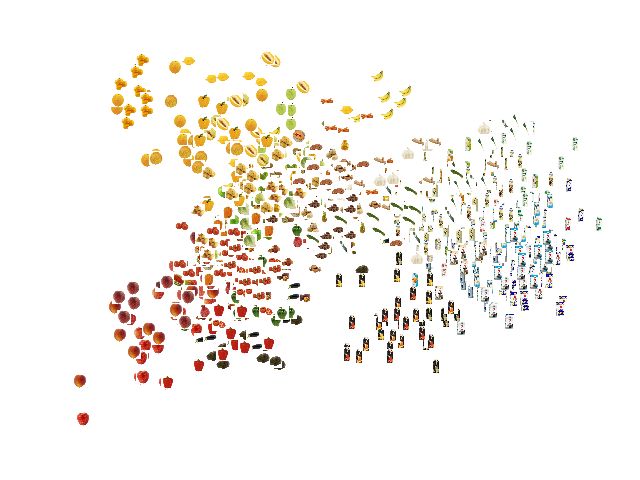
\includegraphics[width=\textwidth]{PaperB/appendix/figures/vcca_private_xi/pca_vcca_xi.png}
			\caption{$\mu_{z}$ from VCCA$_{x i}$}
			\label{fig:pca_vcca_xi_z}
		\end{subfigure}~
		\begin{subfigure}[t]{0.48\textwidth}
			\centering
			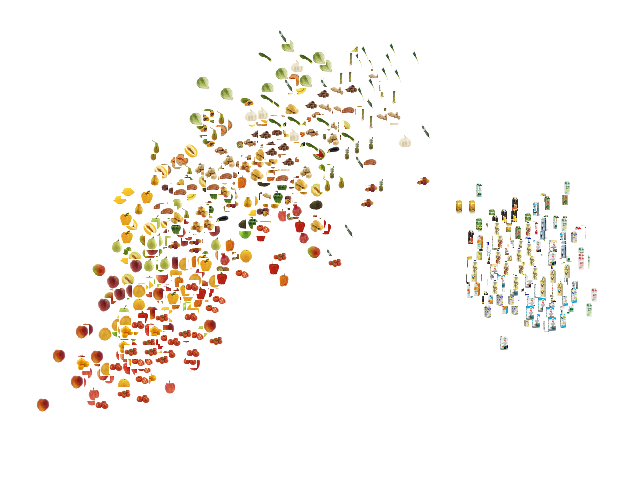
\includegraphics[width=\textwidth]{PaperB/appendix/figures/vcca_private_xi/pca_z_vcca_private_xi_seed1.png}
			\caption{$\mu_{z}$ from VCCA-private$_{x i}$}
			\label{fig:pca_vcca_private_xi_z}
		\end{subfigure}
		%\subfigure[$\mu_{z}$ from VCCA$_{x i}$ ]{\label{fig:pca_vcca_xi_z}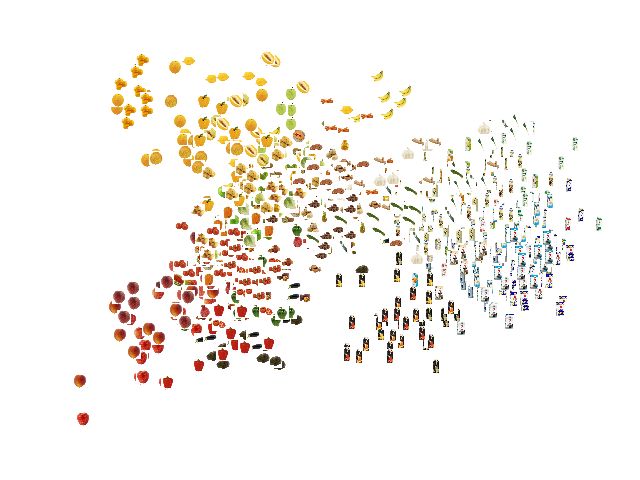
\includegraphics[width=0.45\textwidth]{PaperB/appendix/figures/vcca_private_xi/pca_vcca_xi.png}}~
		%\subfigure[$\mu_{z}$ from VCCA-private$_{x i}$]{\label{fig:pca_vcca_private_xi_z}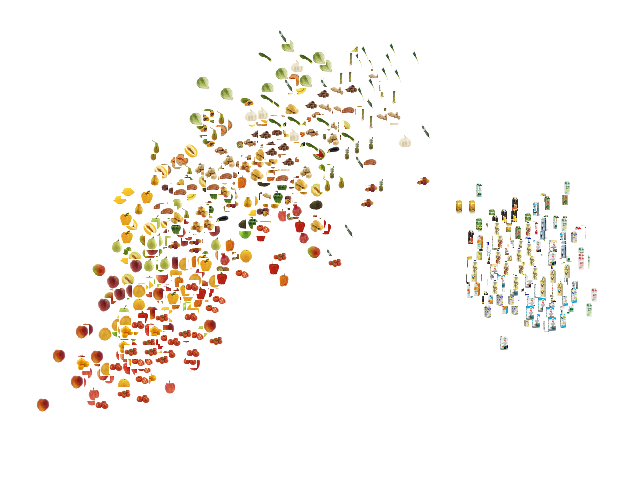
\includegraphics[width=0.45\textwidth]{PaperB/appendix/figures/vcca_private_xi/pca_z_vcca_private_xi_seed1.png}}\\ 
	\end{minipage}
	\begin{minipage}{0.8\textwidth}
		\centering
		\begin{subfigure}[t]{0.6\textwidth}
			\centering
			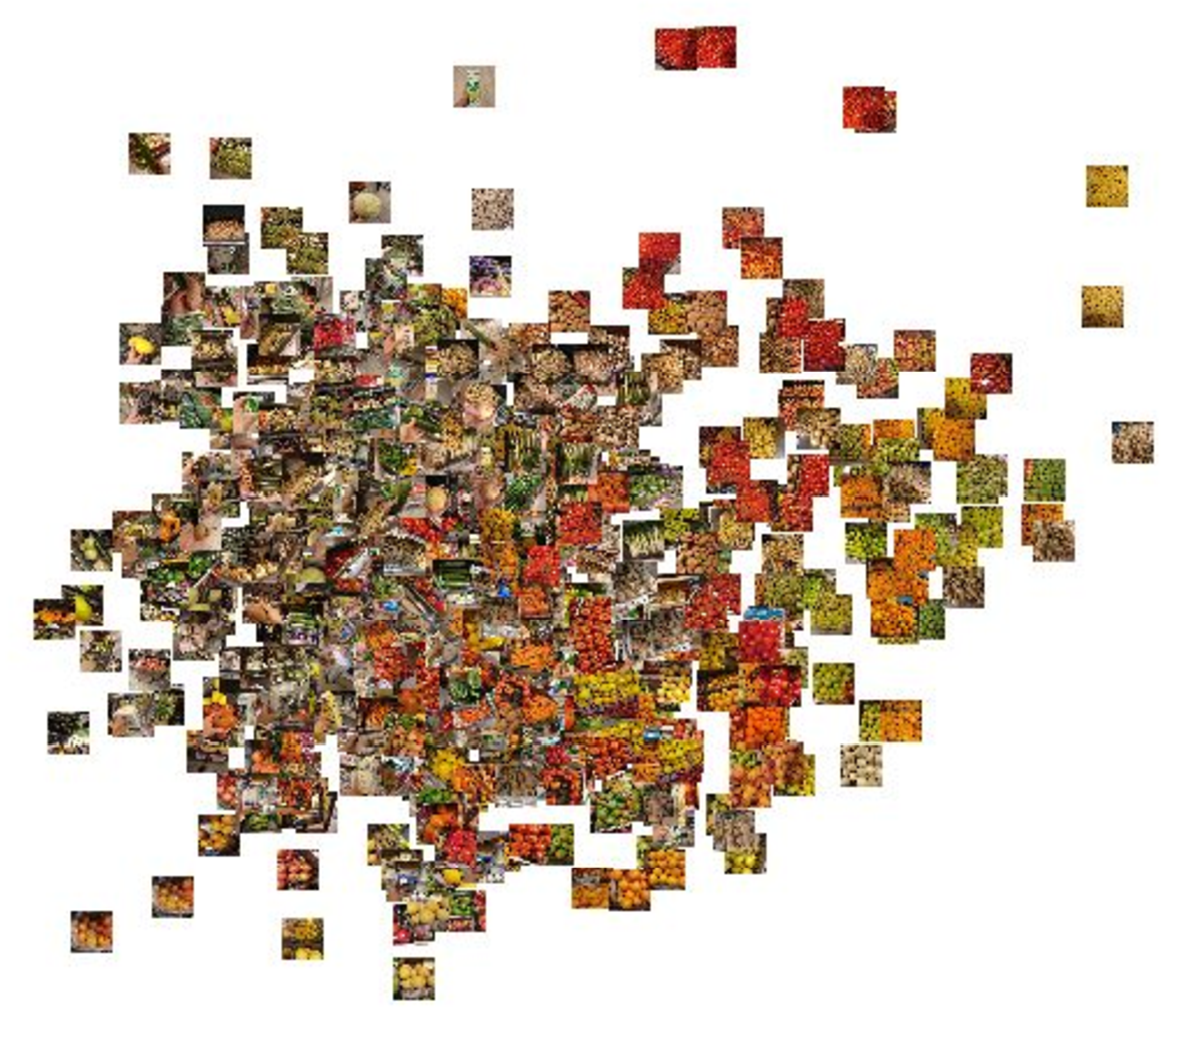
\includegraphics[width=\textwidth]{PaperB/appendix/figures/vcca_private_xi/vcca_private_xi_ux_space.pdf}
			\caption{$\mu_{u_{x}}$ from VCCA-private$_{x i}$}
			\label{fig:pca_vcca_private_xi_ux}
		\end{subfigure} \\
		\begin{subfigure}[t]{0.75\textwidth}
			\centering
			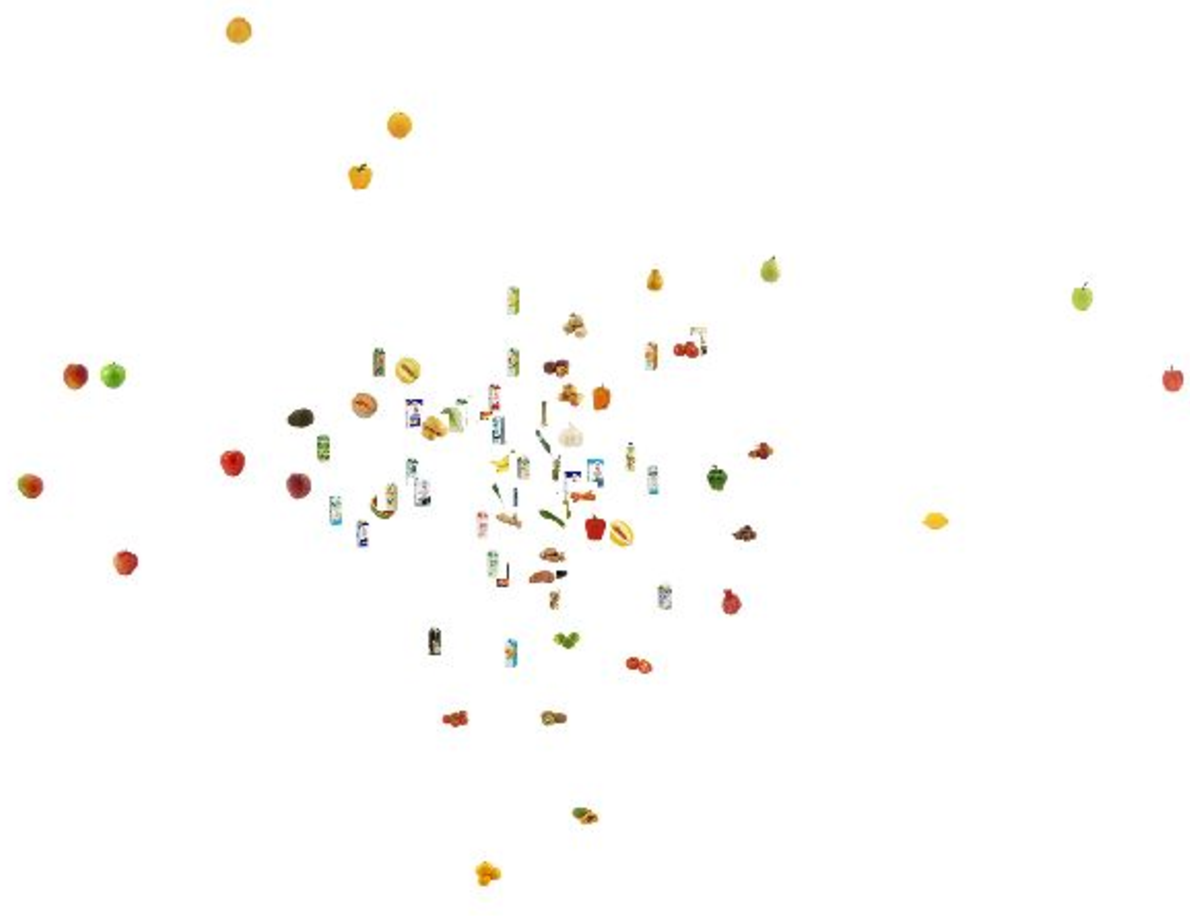
\includegraphics[width=\textwidth]{PaperB/appendix/figures/vcca_private_xi/vcca_private_xi_ui_space.pdf}
			\caption{$\mu_{u_{i}}$ from VCCA-private$_{x i}$}
			\label{fig:pca_vcca_private_xi_ui}
		\end{subfigure}
	\end{minipage}
	\caption{Visualizations of the latent representations $\mu_{z}(x)$ from VCCA$_{x i}$ and VCCA-private$_{x i}$ on the first row followed by $\mu_{u_{x}}(x)$ and $\mu_{u_{i}}(i)$ for VCCA-private$_{x i}$. Abbreviations: VCCA, Variational Canonical Correlation Analysis.}
	\label{paperB:fig:2d_visualizations_pca_vcca_private_xi}
\end{figure}

\clearpage